% Options for packages loaded elsewhere
\PassOptionsToPackage{unicode}{hyperref}
\PassOptionsToPackage{hyphens}{url}
%
\documentclass[
]{article}
\usepackage{amsmath,amssymb}
\usepackage{iftex}
\ifPDFTeX
  \usepackage[T1]{fontenc}
  \usepackage[utf8]{inputenc}
  \usepackage{textcomp} % provide euro and other symbols
\else % if luatex or xetex
  \usepackage{unicode-math} % this also loads fontspec
  \defaultfontfeatures{Scale=MatchLowercase}
  \defaultfontfeatures[\rmfamily]{Ligatures=TeX,Scale=1}
\fi
\usepackage{lmodern}
\ifPDFTeX\else
  % xetex/luatex font selection
\fi
% Use upquote if available, for straight quotes in verbatim environments
\IfFileExists{upquote.sty}{\usepackage{upquote}}{}
\IfFileExists{microtype.sty}{% use microtype if available
  \usepackage[]{microtype}
  \UseMicrotypeSet[protrusion]{basicmath} % disable protrusion for tt fonts
}{}
\makeatletter
\@ifundefined{KOMAClassName}{% if non-KOMA class
  \IfFileExists{parskip.sty}{%
    \usepackage{parskip}
  }{% else
    \setlength{\parindent}{0pt}
    \setlength{\parskip}{6pt plus 2pt minus 1pt}}
}{% if KOMA class
  \KOMAoptions{parskip=half}}
\makeatother
\usepackage{xcolor}
\usepackage[margin=1in]{geometry}
\usepackage{color}
\usepackage{fancyvrb}
\newcommand{\VerbBar}{|}
\newcommand{\VERB}{\Verb[commandchars=\\\{\}]}
\DefineVerbatimEnvironment{Highlighting}{Verbatim}{commandchars=\\\{\}}
% Add ',fontsize=\small' for more characters per line
\usepackage{framed}
\definecolor{shadecolor}{RGB}{248,248,248}
\newenvironment{Shaded}{\begin{snugshade}}{\end{snugshade}}
\newcommand{\AlertTok}[1]{\textcolor[rgb]{0.94,0.16,0.16}{#1}}
\newcommand{\AnnotationTok}[1]{\textcolor[rgb]{0.56,0.35,0.01}{\textbf{\textit{#1}}}}
\newcommand{\AttributeTok}[1]{\textcolor[rgb]{0.13,0.29,0.53}{#1}}
\newcommand{\BaseNTok}[1]{\textcolor[rgb]{0.00,0.00,0.81}{#1}}
\newcommand{\BuiltInTok}[1]{#1}
\newcommand{\CharTok}[1]{\textcolor[rgb]{0.31,0.60,0.02}{#1}}
\newcommand{\CommentTok}[1]{\textcolor[rgb]{0.56,0.35,0.01}{\textit{#1}}}
\newcommand{\CommentVarTok}[1]{\textcolor[rgb]{0.56,0.35,0.01}{\textbf{\textit{#1}}}}
\newcommand{\ConstantTok}[1]{\textcolor[rgb]{0.56,0.35,0.01}{#1}}
\newcommand{\ControlFlowTok}[1]{\textcolor[rgb]{0.13,0.29,0.53}{\textbf{#1}}}
\newcommand{\DataTypeTok}[1]{\textcolor[rgb]{0.13,0.29,0.53}{#1}}
\newcommand{\DecValTok}[1]{\textcolor[rgb]{0.00,0.00,0.81}{#1}}
\newcommand{\DocumentationTok}[1]{\textcolor[rgb]{0.56,0.35,0.01}{\textbf{\textit{#1}}}}
\newcommand{\ErrorTok}[1]{\textcolor[rgb]{0.64,0.00,0.00}{\textbf{#1}}}
\newcommand{\ExtensionTok}[1]{#1}
\newcommand{\FloatTok}[1]{\textcolor[rgb]{0.00,0.00,0.81}{#1}}
\newcommand{\FunctionTok}[1]{\textcolor[rgb]{0.13,0.29,0.53}{\textbf{#1}}}
\newcommand{\ImportTok}[1]{#1}
\newcommand{\InformationTok}[1]{\textcolor[rgb]{0.56,0.35,0.01}{\textbf{\textit{#1}}}}
\newcommand{\KeywordTok}[1]{\textcolor[rgb]{0.13,0.29,0.53}{\textbf{#1}}}
\newcommand{\NormalTok}[1]{#1}
\newcommand{\OperatorTok}[1]{\textcolor[rgb]{0.81,0.36,0.00}{\textbf{#1}}}
\newcommand{\OtherTok}[1]{\textcolor[rgb]{0.56,0.35,0.01}{#1}}
\newcommand{\PreprocessorTok}[1]{\textcolor[rgb]{0.56,0.35,0.01}{\textit{#1}}}
\newcommand{\RegionMarkerTok}[1]{#1}
\newcommand{\SpecialCharTok}[1]{\textcolor[rgb]{0.81,0.36,0.00}{\textbf{#1}}}
\newcommand{\SpecialStringTok}[1]{\textcolor[rgb]{0.31,0.60,0.02}{#1}}
\newcommand{\StringTok}[1]{\textcolor[rgb]{0.31,0.60,0.02}{#1}}
\newcommand{\VariableTok}[1]{\textcolor[rgb]{0.00,0.00,0.00}{#1}}
\newcommand{\VerbatimStringTok}[1]{\textcolor[rgb]{0.31,0.60,0.02}{#1}}
\newcommand{\WarningTok}[1]{\textcolor[rgb]{0.56,0.35,0.01}{\textbf{\textit{#1}}}}
\usepackage{graphicx}
\makeatletter
\def\maxwidth{\ifdim\Gin@nat@width>\linewidth\linewidth\else\Gin@nat@width\fi}
\def\maxheight{\ifdim\Gin@nat@height>\textheight\textheight\else\Gin@nat@height\fi}
\makeatother
% Scale images if necessary, so that they will not overflow the page
% margins by default, and it is still possible to overwrite the defaults
% using explicit options in \includegraphics[width, height, ...]{}
\setkeys{Gin}{width=\maxwidth,height=\maxheight,keepaspectratio}
% Set default figure placement to htbp
\makeatletter
\def\fps@figure{htbp}
\makeatother
\setlength{\emergencystretch}{3em} % prevent overfull lines
\providecommand{\tightlist}{%
  \setlength{\itemsep}{0pt}\setlength{\parskip}{0pt}}
\setcounter{secnumdepth}{-\maxdimen} % remove section numbering
\ifLuaTeX
  \usepackage{selnolig}  % disable illegal ligatures
\fi
\IfFileExists{bookmark.sty}{\usepackage{bookmark}}{\usepackage{hyperref}}
\IfFileExists{xurl.sty}{\usepackage{xurl}}{} % add URL line breaks if available
\urlstyle{same}
\hypersetup{
  pdftitle={Immigration\_EDA},
  pdfauthor={Mario Arce Acosta},
  hidelinks,
  pdfcreator={LaTeX via pandoc}}

\title{Immigration\_EDA}
\author{Mario Arce Acosta}
\date{2024-05-08}

\begin{document}
\maketitle

\begin{Shaded}
\begin{Highlighting}[]
\FunctionTok{library}\NormalTok{(readxl)}
\FunctionTok{library}\NormalTok{(ggplot2)}
\FunctionTok{library}\NormalTok{(forecast)}
\end{Highlighting}
\end{Shaded}

\begin{verbatim}
## Registered S3 method overwritten by 'quantmod':
##   method            from
##   as.zoo.data.frame zoo
\end{verbatim}

\begin{Shaded}
\begin{Highlighting}[]
\CommentTok{\#Path on XCITE laptop"C:\textbackslash{}Users\textbackslash{}XCITE{-}admin\textbackslash{}Documents\textbackslash{}GitHub\textbackslash{}Regular\_R\_Work\textbackslash{}H1B\_data.xlsx"}
\NormalTok{H1B\_data }\OtherTok{\textless{}{-}} \FunctionTok{read\_excel}\NormalTok{(}\StringTok{"C:/Users/mario/Documents/GitHub/Regular\_R\_Work/H1B\_data.xlsx"}\NormalTok{, }\AttributeTok{sheet =} \StringTok{"Sheet 1"}\NormalTok{)}
\FunctionTok{View}\NormalTok{(H1B\_data)}
\NormalTok{LPR\_data }\OtherTok{\textless{}{-}} \FunctionTok{read\_excel}\NormalTok{(}\StringTok{"C:/Users/mario/Documents/GitHub/Regular\_R\_Work/LPR\_1820{-}2022\_data.xlsx"}\NormalTok{, }\AttributeTok{sheet =} \StringTok{"LPR obtainments"}\NormalTok{)}
\FunctionTok{View}\NormalTok{(LPR\_data)}

\NormalTok{fearData}\OtherTok{\textless{}{-}} \FunctionTok{read\_excel}\NormalTok{(}\StringTok{"C:/Users/mario/Desktop/Datasets/Migration\_Fear\_EPU\_Data.xlsx"}\NormalTok{, }\AttributeTok{sheet =} \StringTok{"Sheet1"}\NormalTok{)}
\FunctionTok{View}\NormalTok{(fearData)}

\NormalTok{removalsData }\OtherTok{\textless{}{-}} \FunctionTok{read\_excel}\NormalTok{(}\StringTok{"C:/Users/mario/Desktop/Datasets/Alien\_removal\_returns\_fy2019\_data.xlsx"}\NormalTok{, }\AttributeTok{sheet =} \StringTok{"(R) Aliens removed or returned"}\NormalTok{)}
\FunctionTok{View}\NormalTok{(removalsData)}
\end{Highlighting}
\end{Shaded}

\begin{Shaded}
\begin{Highlighting}[]
\DocumentationTok{\#\#Work began at XCITE}

\CommentTok{\#Prepare H1B\_data}
\FunctionTok{colnames}\NormalTok{(H1B\_data)[}\DecValTok{1}\NormalTok{]}\OtherTok{\textless{}{-}}\StringTok{"Year"}
\FunctionTok{colnames}\NormalTok{(H1B\_data)[}\DecValTok{8}\NormalTok{]}\OtherTok{\textless{}{-}}\StringTok{"Inital\_Approval"}
\FunctionTok{colnames}\NormalTok{(H1B\_data)[}\DecValTok{9}\NormalTok{]}\OtherTok{\textless{}{-}}\StringTok{"Inital\_Denial"}
\FunctionTok{colnames}\NormalTok{(H1B\_data)[}\DecValTok{10}\NormalTok{]}\OtherTok{\textless{}{-}}\StringTok{"Continuing\_Approval"}
\FunctionTok{colnames}\NormalTok{(H1B\_data)[}\DecValTok{11}\NormalTok{]}\OtherTok{\textless{}{-}}\StringTok{"Continuing\_Denial"}

\NormalTok{H1B\_data}\OtherTok{\textless{}{-}}\FunctionTok{subset}\NormalTok{(H1B\_data, Year }\SpecialCharTok{\textless{}=} \DecValTok{2022}\NormalTok{)}

\NormalTok{H1B\_numbers}\OtherTok{\textless{}{-}}\NormalTok{H1B\_data[}\FunctionTok{c}\NormalTok{(}\DecValTok{1}\NormalTok{,}\DecValTok{8}\NormalTok{,}\DecValTok{9}\NormalTok{,}\DecValTok{10}\NormalTok{,}\DecValTok{11}\NormalTok{)]}
\FunctionTok{View}\NormalTok{(H1B\_numbers)}
\NormalTok{H1B\_numbers}\OtherTok{\textless{}{-}}\FunctionTok{aggregate}\NormalTok{(H1B\_numbers[}\DecValTok{2}\SpecialCharTok{:}\DecValTok{5}\NormalTok{],}\AttributeTok{by=}\FunctionTok{list}\NormalTok{(H1B\_numbers}\SpecialCharTok{$}\NormalTok{Year), }\AttributeTok{FUN=}\NormalTok{sum)}

\NormalTok{tsH1B}\OtherTok{\textless{}{-}}\FunctionTok{ts}\NormalTok{(H1B\_numbers}\SpecialCharTok{$}\NormalTok{Continuing\_Approval, }\AttributeTok{start=}\DecValTok{2013}\NormalTok{,}\AttributeTok{end=}\DecValTok{2022}\NormalTok{)}
\FunctionTok{plot.ts}\NormalTok{(tsH1B)}
\end{Highlighting}
\end{Shaded}

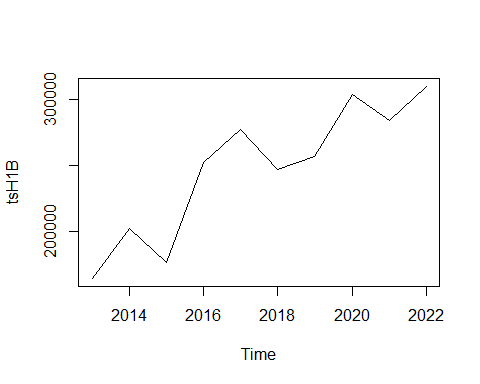
\includegraphics{Immigration_EDA_BUS124B_Mario_files/figure-latex/Clean and Prepare-1.pdf}

\begin{Shaded}
\begin{Highlighting}[]
\CommentTok{\#Prepare LPR\_data by renaming columns, subsetting, and changing data type}
\FunctionTok{colnames}\NormalTok{(LPR\_data)[}\DecValTok{2}\NormalTok{]}\OtherTok{\textless{}{-}}\StringTok{"\#\_of\_LPR\_obtained"}

\NormalTok{tsLPR}\OtherTok{\textless{}{-}}\FunctionTok{ts}\NormalTok{(LPR\_data}\SpecialCharTok{$}\StringTok{\textasciigrave{}}\AttributeTok{\#\_of\_LPR\_obtained}\StringTok{\textasciigrave{}}\NormalTok{,}\AttributeTok{start=}\DecValTok{2013}\NormalTok{,}\AttributeTok{end=}\DecValTok{2022}\NormalTok{, }\AttributeTok{frequency=}\DecValTok{1}\NormalTok{)}
\FunctionTok{plot.ts}\NormalTok{(tsLPR)}
\end{Highlighting}
\end{Shaded}

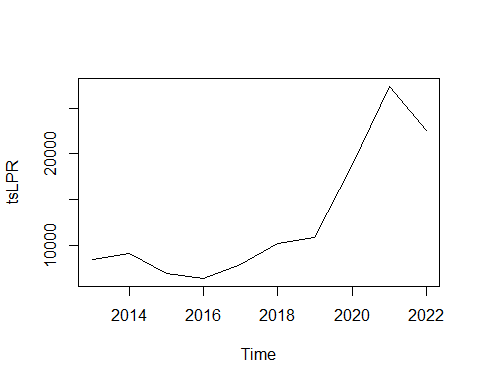
\includegraphics{Immigration_EDA_BUS124B_Mario_files/figure-latex/Clean and Prepare-2.pdf}

\begin{Shaded}
\begin{Highlighting}[]
\NormalTok{LPR\_tsmodel1}\OtherTok{\textless{}{-}}\FunctionTok{tslm}\NormalTok{(tsLPR}\SpecialCharTok{\textasciitilde{}}\NormalTok{trend)}
\FunctionTok{summary}\NormalTok{(LPR\_tsmodel1)}
\end{Highlighting}
\end{Shaded}

\begin{verbatim}
## 
## Call:
## tslm(formula = tsLPR ~ trend)
## 
## Residuals:
##     Min      1Q  Median      3Q     Max 
## -5018.3 -3612.4  -138.1  2720.5  7520.0 
## 
## Coefficients:
##             Estimate Std. Error t value Pr(>|t|)   
## (Intercept)   1831.7     3022.5   0.606  0.56130   
## trend         2003.4      487.1   4.113  0.00338 **
## ---
## Signif. codes:  0 '***' 0.001 '**' 0.01 '*' 0.05 '.' 0.1 ' ' 1
## 
## Residual standard error: 4424 on 8 degrees of freedom
## Multiple R-squared:  0.6789, Adjusted R-squared:  0.6388 
## F-statistic: 16.91 on 1 and 8 DF,  p-value: 0.003378
\end{verbatim}

\begin{Shaded}
\begin{Highlighting}[]
\NormalTok{LPR\_tsmodel2}\OtherTok{\textless{}{-}}\FunctionTok{tslm}\NormalTok{(}\FunctionTok{log}\NormalTok{(tsLPR)}\SpecialCharTok{\textasciitilde{}}\NormalTok{trend)}
\FunctionTok{summary}\NormalTok{(LPR\_tsmodel2)}
\end{Highlighting}
\end{Shaded}

\begin{verbatim}
## 
## Call:
## tslm(formula = log(tsLPR) ~ trend)
## 
## Residuals:
##     Min      1Q  Median      3Q     Max 
## -0.3632 -0.2355 -0.0440  0.2517  0.3867 
## 
## Coefficients:
##             Estimate Std. Error t value Pr(>|t|)    
## (Intercept)   8.5513     0.2023  42.280 1.08e-10 ***
## trend         0.1422     0.0326   4.362  0.00241 ** 
## ---
## Signif. codes:  0 '***' 0.001 '**' 0.01 '*' 0.05 '.' 0.1 ' ' 1
## 
## Residual standard error: 0.2961 on 8 degrees of freedom
## Multiple R-squared:  0.704,  Adjusted R-squared:  0.667 
## F-statistic: 19.03 on 1 and 8 DF,  p-value: 0.002406
\end{verbatim}

\begin{Shaded}
\begin{Highlighting}[]
\CommentTok{\# forecast1\textless{}{-}forecast(LPR\_tsmodel1, h=10)}
\CommentTok{\# forecast2\textless{}{-}forecast(LPR\_tsmodel2, h=10)}
\CommentTok{\# View(forecast1)}
\CommentTok{\# View(forecast2)}
\CommentTok{\# }
\CommentTok{\# exp(forecast2$mean+se\^{}2/2)}

\FunctionTok{ses}\NormalTok{(LPR\_data}\SpecialCharTok{$}\StringTok{\textasciigrave{}}\AttributeTok{\#\_of\_LPR\_obtained}\StringTok{\textasciigrave{}}\NormalTok{, }\AttributeTok{alpha =} \FloatTok{0.3}\NormalTok{)}\SpecialCharTok{$}\NormalTok{fitted}
\end{Highlighting}
\end{Shaded}

\begin{verbatim}
## Time Series:
## Start = 1 
## End = 203 
## Frequency = 1 
##   [1]   10280.160    9711.612    9536.228    8748.660    8030.262    7994.783
##   [7]    8656.048    9310.334   12179.734   16740.414   18474.290   19928.603
##  [13]   20739.922   32662.545   40455.782   47928.547   47162.183   55886.128
##  [19]   62922.290   55719.803   59424.562   66816.993   70858.595   80970.517
##  [25]   72428.162   74284.213   86310.249  106741.974  145209.782  169604.947
##  [31]  207830.663  256475.464  293372.625  316841.737  332382.716  361017.801
##  [37]  312975.561  279213.693  270841.385  226526.769  194953.339  182559.337
##  [43]  155366.936  136352.355  148331.249  161857.274  187736.092  226985.664
##  [49]  253606.565  219176.595  259254.017  297638.712  304752.098  334768.269
##  [55]  372278.688  354596.782  316467.147  272522.803  233323.062  204866.843
##  [61]  196754.590  274905.313  393263.019  511981.714  539383.799  533146.260
##  [67]  491806.182  444525.227  458200.359  484806.951  472692.966  467475.676
##  [73]  495328.673  520628.971  496359.280  433140.796  380759.357  369511.650
##  [79]  327907.755  298325.129  302342.090  346211.063  388723.144  466729.101
##  [85]  583824.171  652537.919  764726.244  865528.871  991474.909  928893.437
##  [91]  875761.206  925503.844  911428.791  889451.754  981983.827 1052932.679
##  [97]  835062.875  674191.813  560555.169  425574.018  340241.413  367169.289
## [103]  498586.902  441877.632  466190.042  538401.829  465175.481  416969.236
## [109]  392430.966  366878.176  340718.123  311012.686  246850.580  183468.206
## [115]  135348.144  103584.701   82996.091   68995.964   63370.374   64727.762
## [121]   70208.833   70372.983   64793.888   53990.022   44910.515   40002.661
## [127]   39437.563   60222.594   86343.416  111611.391  134623.074  168992.252
## [133]  180009.676  205662.773  195094.141  199018.999  210650.299  243942.709
## [139]  268819.997  264153.498  263113.248  263798.674  266062.272  271372.490
## [145]  281838.743  284961.520  288482.164  298849.515  317786.260  358784.782
## [151]  358723.048  363103.933  365316.153  371126.807  379343.265  383715.986
## [157]  384214.590  418678.113  430701.179  478433.825  453176.878  474512.314
## [163]  510662.820  517551.174  527301.422  531654.295  542602.707  559829.995
## [169]  571847.696  592697.187  741939.631  980119.342 1234062.039 1155876.927
## [175] 1080288.649  997399.954  914233.068  914631.148  879595.903  811678.932
## [181]  761611.353  785428.547  867470.583  925036.208  858587.946  888376.462
## [187]  958540.623 1050817.136 1051296.495 1068045.347 1086877.143 1073601.500
## [193] 1070133.050 1058582.435 1038173.604 1031676.923 1037483.146 1081289.702
## [199] 1095052.892 1095520.324 1076393.727  965684.209  897979.546
\end{verbatim}

\begin{Shaded}
\begin{Highlighting}[]
\NormalTok{fittedLPR1}\OtherTok{\textless{}{-}}\FunctionTok{fitted}\NormalTok{(LPR\_tsmodel1)}
\FunctionTok{accuracy}\NormalTok{(}\FunctionTok{fitted}\NormalTok{(LPR\_tsmodel1),LPR\_data}\SpecialCharTok{$}\StringTok{\textasciigrave{}}\AttributeTok{\#\_of\_LPR\_obtained}\StringTok{\textasciigrave{}}\NormalTok{[}\DecValTok{1}\SpecialCharTok{:}\DecValTok{10}\NormalTok{])}
\end{Highlighting}
\end{Shaded}

\begin{verbatim}
##                     ME     RMSE      MAE       MPE     MAPE
## Test set -1.818268e-13 3957.349 3405.915 -7.423898 32.63382
\end{verbatim}

\begin{Shaded}
\begin{Highlighting}[]
\NormalTok{se}\OtherTok{\textless{}{-}}\FunctionTok{sigma}\NormalTok{(LPR\_tsmodel2)}
\FunctionTok{accuracy}\NormalTok{(}\FunctionTok{fitted}\NormalTok{(LPR\_tsmodel2)}\SpecialCharTok{+}\NormalTok{se}\SpecialCharTok{\^{}}\DecValTok{2}\NormalTok{,LPR\_data}\SpecialCharTok{$}\StringTok{\textasciigrave{}}\AttributeTok{\#\_of\_LPR\_obtained}\StringTok{\textasciigrave{}}\NormalTok{[}\DecValTok{1}\SpecialCharTok{:}\DecValTok{10}\NormalTok{])}
\end{Highlighting}
\end{Shaded}

\begin{verbatim}
##                ME     RMSE      MAE      MPE     MAPE
## Test set 12840.78 14616.87 12840.78 99.90886 99.90886
\end{verbatim}

\begin{Shaded}
\begin{Highlighting}[]
\CommentTok{\#Prepare crimeData by subsetting and changing data type}
\NormalTok{removalsData }\OtherTok{\textless{}{-}}\NormalTok{removalsData[}\DecValTok{99}\SpecialCharTok{:}\DecValTok{128}\NormalTok{,]}
\NormalTok{removalsData}\SpecialCharTok{$}\NormalTok{Year }\OtherTok{\textless{}{-}} \FunctionTok{as.numeric}\NormalTok{(removalsData}\SpecialCharTok{$}\NormalTok{Year)}
\end{Highlighting}
\end{Shaded}

\begin{verbatim}
## Warning: NAs introduced by coercion
\end{verbatim}

\begin{Shaded}
\begin{Highlighting}[]
\CommentTok{\#Prepare fearData by subsetting, aggregating, and renaming columns}
\NormalTok{fearData }\OtherTok{\textless{}{-}}\NormalTok{ fearData[}\FunctionTok{c}\NormalTok{(}\DecValTok{1}\NormalTok{,}\DecValTok{2}\NormalTok{,}\DecValTok{7}\NormalTok{,}\DecValTok{8}\NormalTok{)]}
\NormalTok{tsFear}\OtherTok{\textless{}{-}}\FunctionTok{ts}\NormalTok{(fearData}\SpecialCharTok{$}\NormalTok{usa\_fear\_index, }\AttributeTok{frequency=}\DecValTok{4}\NormalTok{)}
\NormalTok{tsMigrant}\OtherTok{\textless{}{-}}\FunctionTok{ts}\NormalTok{(fearData}\SpecialCharTok{$}\NormalTok{usa\_epu\_migrant\_index, }\AttributeTok{frequency=}\DecValTok{4}\NormalTok{)}

\FunctionTok{plot.ts}\NormalTok{(tsFear)}
\end{Highlighting}
\end{Shaded}

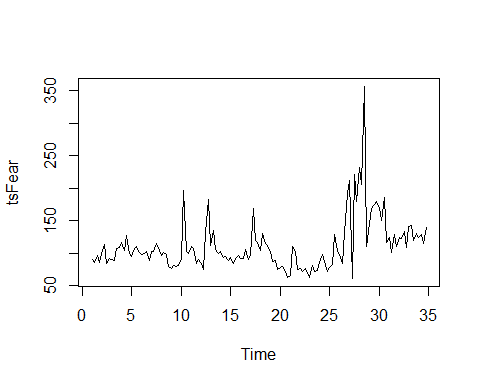
\includegraphics{Immigration_EDA_BUS124B_Mario_files/figure-latex/Clean and Prepare-3.pdf}

\begin{Shaded}
\begin{Highlighting}[]
\FunctionTok{plot.ts}\NormalTok{(tsMigrant)}
\end{Highlighting}
\end{Shaded}

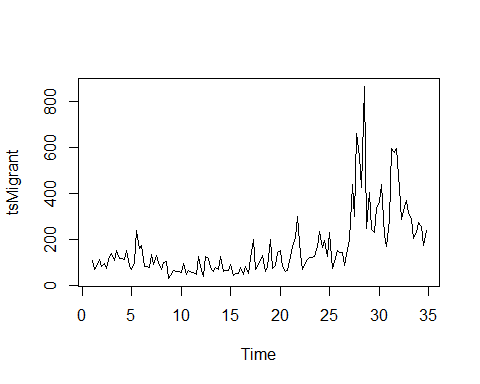
\includegraphics{Immigration_EDA_BUS124B_Mario_files/figure-latex/Clean and Prepare-4.pdf}

\begin{Shaded}
\begin{Highlighting}[]
\NormalTok{fearData}\OtherTok{\textless{}{-}}\FunctionTok{aggregate}\NormalTok{(fearData,}\AttributeTok{by=}\FunctionTok{list}\NormalTok{(fearData}\SpecialCharTok{$}\NormalTok{year), }\AttributeTok{FUN=}\NormalTok{ mean)}
\NormalTok{fearData}\OtherTok{\textless{}{-}}\NormalTok{fearData[}\DecValTok{2}\SpecialCharTok{:}\DecValTok{4}\NormalTok{]}
\NormalTok{fearData}\OtherTok{\textless{}{-}}\NormalTok{fearData[}\DecValTok{1}\SpecialCharTok{:}\DecValTok{30}\NormalTok{,]}
\FunctionTok{colnames}\NormalTok{(fearData)[}\DecValTok{1}\NormalTok{] }\OtherTok{\textless{}{-}} \StringTok{"Year"}

\CommentTok{\#Merge into a single dataframe with all column headers}
\CommentTok{\# immigrationData \textless{}{-} merge(removalsData,lprData)}
\CommentTok{\# immigrationData \textless{}{-} merge(immigrationData, fearData)}
\CommentTok{\# View(immigrationData)}
\end{Highlighting}
\end{Shaded}

\begin{Shaded}
\begin{Highlighting}[]
\CommentTok{\# \#Plots by data sources for now}
\CommentTok{\# ggplot(fearData, aes(Year, usa\_fear\_index)) + }
\CommentTok{\#   geom\_point() + geom\_line()}
\CommentTok{\# ggplot(lprData, aes(Year, Persons\_obtaining\_LPR)) + }
\CommentTok{\#   geom\_point() + geom\_line()}
\CommentTok{\# ggplot(removalsData, aes(Year, Removals1)) + }
\CommentTok{\#   geom\_point() + geom\_line()}
\CommentTok{\# }
\CommentTok{\# \#model1\textless{}{-} lm(Removals1 \textasciitilde{} usa\_fear\_index , immigrationData)}
\CommentTok{\#model2\textless{}{-} lm(usa\_epu\_migrant\_index \textasciitilde{} usa\_fear\_index, fearData)}
\CommentTok{\# \#model3\textless{}{-} lm(Persons\_obtaining\_LPR\textasciitilde{}usa\_fear\_index, fearData)}
\CommentTok{\# \#summary(model1)}
\CommentTok{\#summary(model2)}
\CommentTok{\# \#summary(model3)}
\end{Highlighting}
\end{Shaded}

\hypertarget{r-markdown}{%
\subsection{R Markdown}\label{r-markdown}}

This is an R Markdown document. Markdown is a simple formatting syntax
for authoring HTML, PDF, and MS Word documents. For more details on
using R Markdown see \url{http://rmarkdown.rstudio.com}.

When you click the \textbf{Knit} button a document will be generated
that includes both content as well as the output of any embedded R code
chunks within the document. You can embed an R code chunk like this:

Note that the \texttt{echo\ =\ FALSE} parameter was added to the code
chunk to prevent printing of the R code that generated the plot.

\end{document}
